\documentclass[12pt,a4paper,oneside]{book}

\usepackage{amsmath}
\usepackage{amssymb}
\usepackage{amsthm}
\usepackage{graphicx}
\usepackage{latexsym}
%\usepackage{pslatex}
\usepackage{color}
\usepackage{fancyhdr}
\usepackage{cite}
\usepackage{indentfirst}
\usepackage{tocloft}
\usepackage{multirow}
\usepackage{fontspec}
\usepackage{hyperref}
\usepackage{pdfpages}
%\setmainfont{Times New Roman}

% Centering Chapter
\usepackage{sectsty}
\chapterfont{\centering}

\pagestyle{myheadings}
\setlength{\parindent}{0.8in}

\usepackage[top=1.5in,bottom=1in,left=1in,right=1in]{geometry}

% Theorem style-------------------------------------------------------------------
\theoremstyle{plain}
\newtheorem{thm}{Theorem}[chapter]
\newtheorem{lem}[thm]{Lemma}
\newtheorem{cor}[thm]{Corollary}
\newtheorem{prop}[thm]{Proposition}
\newtheorem{rem}[thm]{Remark}
\newtheorem{ex}[thm]{Example}
\newtheorem{de}[thm]{Definition}

\numberwithin{equation}{chapter}
\DeclareMathOperator{\Var}{Var}
\DeclareMathOperator{\Ima}{Im}

\usepackage{float}
%\usepackage[skip=2pt,font=footnotesize]{caption}

% Graph-------------------------------------------------------------------
\usepackage{graphics,graphicx}
\usepackage{calc}
\usepackage{tikz}
\usetikzlibrary{decorations.markings, fit, positioning, arrows.meta, backgrounds}
\tikzstyle{vertex}=[circle, draw, inner sep=2pt, minimum size=4pt]
\usepackage{circuitikz}
\newcommand{\vertex}{\node[vertex]}
\newcounter{Angle}
\usepackage{pgfgantt}

% Line space-------------------------------------------------------------------
\renewcommand{\baselinestretch}{1.5}


%Centering table of contents and list of table
\usepackage{tocloft}
\renewcommand{\contentsname}{\hfill\bfseries\Large TABLE OF CONTENTS \hfill}
\renewcommand{\cftaftertoctitle}{\hfill}

\renewcommand{\listtablename}{\hfill\bfseries\Large LIST OF TABLES}
\renewcommand{\cftafterlottitle}{\hfill}

\renewcommand{\listfigurename}{\hfill\bfseries\Large LIST OF FIGURES}
\renewcommand{\cftafterloftitle}{\hfill}

\renewcommand*\thesection{\arabic{section}}

\begin{document}

\thispagestyle{empty}

\begin{figure}[h!]
\vskip1in
\begin{center}

\includegraphics[width = 3.5 cm]{res/DCU_logo_square.png}
\end{center}
\end{figure}

\begin{center}
\large\textbf{Glovesy}
\end{center}

\vskip2.5cm

\begin{center}
\textbf{BY}
\end{center}

\vskip0.6cm

\begin{center}
\textbf{Alan Devine - 17412402}\\
\textbf{Sean Moloney - 17477122}
\end{center}

\vskip3.5cm

\begin{center}
\textbf{A functional specification document}
\end{center}

\begin{center}
\textbf{As a requirement for CA400}
\end{center}
\vskip2cm
\begin{center}
\textbf{Dublin City University (DCU)}
\end{center}

\newpage
\pagenumbering{roman}
\begin{center}
    \large\textbf{Plagiarism Declaration}
\end{center}
\noindent I/We declare that this material, which I/We now submit for assessment, is entirely my/our own work and has not been taken from the work of others, save and to the extent that such work has been cited and acknowledged within the text of my/our work. I/We understand that plagiarism, collusion, and copying are grave and serious offences in the university and accept the penalties that would be imposed should I/We engage in plagiarism, collusion, or copying. I/We have read and understood the Assignment Regulations. I/We have identified and included the source of all facts, ideas, opinions, and viewpoints of others in the assignment references. Direct quotations from books, journal articles, internet sources, module text, or any other source whatsoever are acknowledged and the source cited are identified in the assignment refernces. This assignment, or any part of it, has not been previously submitted by me/us or any other person for assessment on this or any other course of study. \\
\\
I/We have read and understood the referencing guidelines found at \\
\url{https://www.dcu.ie/info/regulations/plagiarism.shtml}, \\
\url{https://www4.dcu.ie/students/az/plagiarism}, \\
and/or recommended in the assignment guidelines.

\pagenumbering{roman}
\begin{table}[h]
	\begin{tabular}{ll}
		Project Title								   & Glovesy  \\
		By							   					  & Alan Devine - 17412402\\
															& Sean Moloney - 17477122\\
		Field of Study			  					 & Computer science \\
		Project Advisor								& David Sinclair \\
		Academic Years							  & 2020/2021 \\
	\end{tabular}
\end{table}

\newpage

\begin{center}
  \large\textbf{ABSTRACT}\\
\end{center}
\addcontentsline{toc}{chapter}{ABSTRACT}
\noindent Glovesy is a wearable computer interfacing device in the form of glove which will allow the user to interface with their computer by using custom macros, or use the device for hand-tracking in VR or AR applications. \\
\noindent \textbf{Keywords:} : Wearables, human-computer interfacing, VR, AR, Arduino


%\renewcommand{\contentsname}{TABLE OF CONTENTS}

\newpage
\tableofcontents

%\newpage
%\addcontentsline{toc}{chapter}{LIST OF FIGURES}
%\listoffigures

\newpage
\pagenumbering{arabic}
\chapter*{Introduction}
\addcontentsline{toc}{chapter}{Introduction}

\noindent Glovesy is a wearable device which will allow the user to inteface with their computer, either by using user-defined macros, which will be set up using our program which will allow a number of gestures do be defined to certain actions within the PC, or by allowing the user accurate hand and finger tracking for use in Virtual and Augmented Reality.
\vspace{2cm}

\chapter*{General Description}
\addcontentsline{toc}{chapter}{General Description}

\section{Product / System Functions}

\noindent Glovesy is a wearable human/computer interacing device, which will allow users to interact with their PC in a number of different ways, for different scopes.  The primary focus of the device, will be to allow the user to set up macros, or certain movements or gestures, which the computer will recognise as a specific command, thereby allowing ease of use. Another function of the device will be to track user hand and finger movements for increased accuracy and control in VR applications, since the device is so low profile, as opposed to current VR controllers which tend to be bulky, handheld devices.

\section{User Characteristics and Objectives}

\noindent Glovesy is designed for users who engage in VR/AR applications. This includes, but is not limited to, Gaming, Product prototyping across remote teams,  Creating virtual art, etc. In addition to VR/AR users, given that Glovesy is designed to be a standard input device, we also envision it being used in environments such as,  a presenter navigating a stage, users who for whatever reason may not feel comfortable/can use traditional input devices, etc. We hope to make Glovesy as accessible as possible to the vast majority of users, that being said, here is our idea of the "Ideal User".

\begin{itemize}
    \item Experience with gesture-based input devices
    \begin{itemize}
        \item e.g. Nintendo Wii, or an Air mouse.
    \end{itemize}
    \item Experience with defining Macros
    \begin{itemize}
        \item Keyboard and Mouse Combinations that are present with devices with extra additional keys/ buttons.
    \end{itemize}
\end{itemize}

\section{Operational Scenarios}

\begin{enumerate}
\item \textbf{Gaming in a VR setting:}
\begin{itemize}
    \item The User would see a virtual representation of their hand (this is entirely dependent on the Game itself). The user would be able to interact with their surroundings using Gloves rather than a traditional controller.
\end{itemize}

\item \textbf{Using an AR Device:}
\begin{itemize}
    \item The User would be able to control their AR Device using hand gestures.
\end{itemize}


\item \textbf{Mouse Emulation:}
\begin{itemize}
    \item Within a normal desktop, a User would be able to control their mouse cursor by moving their hand in a way similar to the WiiMote. The user would be able to left click by tensing their index finger and right click using their middle finger.
\end{itemize}


\item \textbf{Gesture Control:}
\begin{itemize}
    \item The User would define some sequence of hand movement combined with finger position, and create a mapping to certain actions on their computer, e.g. raising and lowering system volume, advancing slides, etc.
\end{itemize}

\end{enumerate}

\section{Constraints}

\noindent There are a number of constraints that we foresee will have some impact on the development process of this project.

\begin{itemize}
    \item \textbf{Distinguishing Gestures:} It may be challenging to distinguish hand movements between general movement and purposeful gestures.
    \item \textbf{Application Support:} It could be difficult to set up programs to use the device, as, particularly in games, there may be different controls that are pre-defined.
    \item \textbf{Cross-platform:} a different driver will need to be made for different operating systems, which could be challenging.
\end{itemize}

\chapter*{Functional Requirements}
\addcontentsline{toc}{chapter}{Functional Requirements}


\section{\textbf{Hand Tracking}}

\noindent The device must be able to track the overall hand's orientation and position in 3D space.


\begin{itemize}
    \item \textbf{Criticality:} This aspect is quite important to the overall accuracy of the device, especially for tracking the hand for VR and for Gesture Recognition.
    \item \textbf{Technical Issues:} A significant issue with this is that the accuracy is almost entirely dependent on the hardware, meaning if the IMU device we use is innacruate, we wont be able to do anything to improve the tracking.
\end{itemize}


\section{\textbf{Finger Tracking}}

\noindent The device must be able to track the fingers' individual joints accurately.

\begin{itemize}
    \item \textbf{Criticality:} This aspect is also quite important, as it is one of the main functions of the device.
    \item \textbf{Technical Issues:} One of the main issues with this is that the flex sensors that we are using are made by us, so there will need to be some calibration when first using the device.
\end{itemize}


\newpage


\section{\textbf{Data Transfer}}

\noindent The device must be able to transfer data to the PC reliably.

\begin{itemize}
    \item \textbf{Criticality} This Aspect is very important, since, even if the rest of the data is accurately measured, if the data isn't transferred reliably, the device is useless.
    \item \textbf{Technical Issues:} One of the issues with this will be getting the bluetooth module on the board we are using to be reliable, otherwise we can use the device with
\end{itemize}


\section{\textbf{Gesture Recognition}}

\noindent The system must be able to distinguish between random movements and intentional gestures.

\begin{itemize}
    \item \textbf{Criticality:} This requirement is important for a specific use-case scenario which is not focused on gaming or vr, but rather on workflow.
    \item \textbf{Technical Issues:} Due to the nature of the device, we only have a certain number of inputs, and thereby limited on the amount of information we get from the device, meaning that we will have to focus on some way to distinguish between gestures and non-gestures through pattern recogntition.
\end{itemize}


\chapter*{System Architecture}
\addcontentsline{toc}{chapter}{System Architecture}

\begin{figure}[h!]
    \begin{tikzpicture}
        \node[] (ard) {Arduino};
        \node[above=of ard] (imu) {IMU};
        \node[below=of ard] (fn) {...};
        \node[left=of fn] (f1) {Flex 1};
        \node[right=of fn] (f8) {Flex 8};

        \node[fit=(f1) (fn) (f8), draw, inner sep=5mm] (fit3) {};

        \draw [->] (fit3)--(ard);
        \draw [->] (imu)--(ard);

        \node[fit=(ard) (imu) (fit3), draw, inner sep=5mm] (glove) {};

        \node[below=of glove] (btr) {Bluetooth Reciever};
        \draw [->] (glove)--(btr);

        \node[below=of btr] (driver) {Device Driver};
        \draw [->] (btr)--(driver);

        \node[below=of driver] (daemon) {Daemon};
        \draw [->] (driver)--(daemon);


        \node[right=of daemon] (gui) {GCS};
        \draw [->] (daemon)--(gui);

        \node[below=of daemon] (macro) {MacroDB};
        \draw [->] (gui)|-(macro);
        \draw [->] (macro)--(daemon);

        \node[left=of daemon] (host) {General Input};
        \draw [->] (daemon)--(host);

        \node[fit=(btr) (driver) (daemon) (host) (gui) (macro), draw, inner sep=5mm] (host) {};

        \node[left=of host] (hostLable) {Host Computer};
        \node[left=of glove] (hostLable) {Glovesy};
    \end{tikzpicture}
    \caption{High-Level System Architecture Diagram}
    \label{fig:sys-arch diagram}
\end{figure}

\newpage
\section{Arduino}

\noindent The arduino in use is an *Adafruit Feather M0 Bluefruit*. This has an integreated Bluetooth controler which allows us to transfer data to and from the host computer. This Arduino has 10 analog pins which we can use to measure resistance on our flex sensors.

\section{Flex sensor Array}

\noindent A flex sensor is a vairable resistor that changes resistence based on how much the sensor is bent. For this project we will be making use of 8 flex sensors which will measure the position of each knuckle as well as each finger joint. With the exception of the Thumb and pinky fingers, which will only have one flex sensor each. To help mitigate the costs associated with this project, we will be constructing our own flex sensors using several layers of velostat and conductive thread which will act as our positive and negative terminals.

\section{IMU}

\noindent The IMU, or Inertial measurement unit is the device which we will use to measure the device in 3D space. Our device in question, measures Acceleration and Gyroscopic data on the X, Y and Z Axises in meters per second and radians respectivly. Our IMU also measures temperature, however that will not be used for this project.

\section{Macro Database}

\noindent User defined macros will be stored in a database implemented in MongoDB. We chose MongoDB as conceptually, it makes more sense to group these actions as an object rather than in a relational database.

\chapter*{High-Level Design}
\addcontentsline{toc}{chapter}{High-Level Design}

\begin{figure}[h!]
    \centering
    \begin{tikzpicture}[
            every matrix/.style={ampersand replacement=\&,column sep=2cm,row sep=.6cm},
            source/.style={draw, thick, rounded corners, fill=yellow!20,inner sep=.3cm},
            to/.style={->,>=stealth',shorten >=1pt,semithick,font=\rmfamily\scriptsize},
            every node/.style={align=center}]
        \matrix{%
            \node[source, label=left:Flex Sensors] (A) {A}; \& \& \& \node[source, label=right:Configuration Suite] (B) {B}; \\
            \\\\\\
            \node[source, label=left:Feather Board] (C) {C}; \& \& \node[source, label=below:Driver] (D) {D}; \\
            \\\\\\
            \node[source, label=left:IMU] (F) {F}; \& \& \& \node[source, label=right:Visualiser] (E) {E}; \\
        };

        \draw[->] (A) -- node[anchor=west] {Flex State} (C);
        \draw[->] (F) -- node[anchor=west] {IMU Position} (C);
        \draw[->] (C) -- node[anchor=south] {IMU and Flex Data} (D);
        \draw[->] (D) -| node[anchor=west] {Standardized Data} (B);
        \draw[->] (D) -| (E);

        \node[draw,dotted,fit=(A) (C) (F),inner sep=4ex,] (ACF) {};
        \node[above of =ACF] (ACFt) [above=-5ex of ACF] {Glove};
        \node[draw, dotted,fit=(D) (B) (E), inner sep=5ex] (DBE) {};
        \node[above of = DBE] (DBEt) [above=-5ex of DBE] {PC};
        \node[draw, dotted, fit=(B) (E), inner sep=1ex] (BE) {};
        \node[above of = BE] (BEt) [above=-5ex of BE] {UI};
    \end{tikzpicture}
    \caption{Data Flow Diagram}
    \label{fig:DFD}
\end{figure}

\begin{figure}[h!]
    \centering
    \begin{circuitikz}
        \ctikzset{multipoles/dipchip/width=2};
        \ctikzset{multipoles/dipchip/pin spacing=.2};
        \draw (8,6) node[dipchip, num pins=10,hide numbers, external pins width=0] (IMU) {\footnotesize IMU};
        \draw (8,2) node[dipchip, num pins=32,hide numbers, external pins width=0] (Main) {\footnotesize Feather M0};
        \draw (0,0) node[dipchip, num pins=4, hide numbers, external pins width=0] (Flex1) {};
        \draw (0,1) node[dipchip, num pins=4, hide numbers, external pins width=0] (Flex2) {};
        \draw (0,2) node[dipchip, num pins=4, hide numbers, external pins width=0] (Flex3) {};
        \draw (0,3) node[dipchip, num pins=4, hide numbers, external pins width=0] (Flex4) {};
        \draw (0,4) node[dipchip, num pins=4, hide numbers, external pins width=0] (Flex5) {};
        \draw (0,5) node[dipchip, num pins=4, hide numbers, external pins width=0] (Flex6) {};
        \draw (0,6) node[dipchip, num pins=4, hide numbers, external pins width=0] (Flex7) {};
        \draw (0,7) node[dipchip, num pins=4, hide numbers, external pins width=0] (Flex8) {};

        \node[right, font=\tiny] at (Main.bpin 2) {3V};
        \node[right, font=\tiny] at (Main.bpin 4) {GND};
        \node[right, font=\tiny] at (Main.bpin 5) {A0};
        \node[right, font=\tiny] at (Main.bpin 6) {A1};
        \node[right, font=\tiny] at (Main.bpin 7) {A2};
        \node[right, font=\tiny] at (Main.bpin 8) {A3};
        \node[right, font=\tiny] at (Main.bpin 9) {A4};
        \node[right, font=\tiny] at (Main.bpin 10) {A5};
        \node[left, font=\tiny] at (Main.bpin 29) {13};
        \node[left, font=\tiny] at (Main.bpin 27) {11};
        \node[left, font=\tiny] at (Main.bpin 25) {9};
        \node[left, font=\tiny] at (Main.bpin 22) {SCL};
        \node[left, font=\tiny] at (Main.bpin 21) {SDA};
        
        \node[right, font=\tiny] at (IMU.bpin 1) {VIN};
        \node[right, font=\tiny] at (IMU.bpin 3) {GND};
        \node[right, font=\tiny] at (IMU.bpin 4) {SCL};
        \node[right, font=\tiny] at (IMU.bpin 5) {SDA};

        \node[left, font=\tiny] at (Flex1.bpin 4) {+};
        \node[left, font=\tiny] at (Flex1.bpin 3) {-};

        \node[left, font=\tiny] at (Flex2.bpin 4) {+};
        \node[left, font=\tiny] at (Flex2.bpin 3) {-};

        \node[left, font=\tiny] at (Flex3.bpin 4) {+};
        \node[left, font=\tiny] at (Flex3.bpin 3) {-};

        \node[left, font=\tiny] at (Flex4.bpin 4) {+};
        \node[left, font=\tiny] at (Flex4.bpin 3) {-};

        \node[left, font=\tiny] at (Flex5.bpin 4) {+};
        \node[left, font=\tiny] at (Flex5.bpin 3) {-};

        \node[left, font=\tiny] at (Flex6.bpin 4) {+};
        \node[left, font=\tiny] at (Flex6.bpin 3) {-};

        \node[left, font=\tiny] at (Flex7.bpin 4) {+};
        \node[left, font=\tiny] at (Flex7.bpin 3) {-};

        \node[left, font=\tiny] at (Flex8.bpin 4) {+};
        \node[left, font=\tiny] at (Flex8.bpin 3) {-};

        \node[draw,dotted,fit=(Flex1) (Flex2) (Flex3) (Flex4) (Flex5) (Flex6) (Flex7) (Flex8),inner sep=3ex] (FlexBox) {};
        \node[above of=Flex8] (FlexBoxText) [above=-2ex of Flex8] {Flex Sensors};


        \draw (Main.pin 2) -- + (-1.5,0) node[circ](IMUv){} |- (IMU.pin 1);
        \draw (Main.pin 4) -- + (-2,0) node[circ](gnd){} |- (IMU.pin 3); 
        \draw (Main.pin 22) -- + (.5,0) -- + (.5,3.2) -- + (-3.6,3.2) |- (IMU.pin 4);
        \draw (Main.pin 21) -- + (.8,0) -- + (.8, 3.8) -- + (-3.3, 3.8) |- (IMU.pin 5);


        \draw (Flex1.pin 3) -- + (1,0) node[circ](gflex){} -- + (3.2,0) node[circ](groundflex){};
        \draw (Flex2.pin 3) -- + (1,0) node[circ]{};
        \draw (Flex3.pin 3) -- + (1,0) node[circ]{};
        \draw (Flex4.pin 3) -- + (1,0) node[circ]{};
        \draw (Flex5.pin 3) -- + (1,0) node[circ]{};
        \draw (Flex6.pin 3) -- + (1,0) node[circ]{};
        \draw (Flex7.pin 3) -- + (1,0) node[circ]{};
        \draw (Flex8.pin 3) -- + (1,0) -- (gflex);


        \draw (gnd) -- (groundflex);

        \draw (Flex1.pin 4) -- + (1.5,0) node[circ](vflex){} -| (IMUv);
        \draw (Flex2.pin 4) -- + (1.5,0) node[circ]{};
        \draw (Flex3.pin 4) -- + (1.5,0) node[circ]{};
        \draw (Flex4.pin 4) -- + (1.5,0) node[circ]{};
        \draw (Flex5.pin 4) -- + (1.5,0) node[circ]{};
        \draw (Flex6.pin 4) -- + (1.5,0) node[circ]{};
        \draw (Flex7.pin 4) -- + (1.5,0) node[circ]{};
        \draw (Flex8.pin 4) -- + (1.5,0) -- (vflex);

        \draw (Main.pin 5) -- + (-1,0) node[circ](a0){};
        \draw (Main.pin 6) -- + (-1,0) node[circ](a1){};
        \draw (Main.pin 7) -- + (-1,0) node[circ](a2){};
        \draw (Main.pin 8) -- + (-1,0) node[circ](a3){};
        \draw (Main.pin 9) -- + (-1,0) node[circ](a4){};
        \draw (Main.pin 10) -- + (-1,0) node[circ](a5){};

        \draw (Main.pin 27) -- + (1.3,0) node[circ](11){};
        \draw (Main.pin 25) -- + (1.3,0) node[circ](9){};

        \draw (Main.pin 29) -- + (1.3,0) -- (11);
        \draw (groundflex) -| (a0);
        \draw (groundflex) -- + (0,-.5) -| (11);

    \end{circuitikz}
    \caption{Circuit Diagram}
    \label{fig:Circuit}
\end{figure}

\begin{figure}[h!]
    \centering
    \begin{circuitikz}
        \tikzset={>=latex};
        \draw (2, 0) node[resistivesensshape](r){};
        \draw[->,>=stealth] (r.label) -- + (.49, .9);

        \draw (r.east) -- + (1.5,0) node[ocirc](vin){};
        \node [above of=vin] [above=-5ex of vin]{V\footnotesize in};

        \draw (0,-1.5) node[resistorshape, rotate=90](pullup){};

        \draw (pullup.east) -- + (0,.93) node[circ](a){};
        \draw (a) -- (r.west);
        \draw (a) -- + (-1,0) node[ocirc](vout){};
        \draw (pullup.west) -- + (0,-.5) node[ground]{};

        \node[above of=vout] [above=-5ex of vout] {V\footnotesize out};

        \node[above of=r] {\footnotesize Flex Sensor};
        \node[left of=pullup] {\footnotesize 4.7 \tiny k $\Omega$};
    \end{circuitikz}
    \caption{Flex Sensor Circuit}
    \label{fig:flex}
\end{figure}

\begin{figure}
    \centering
    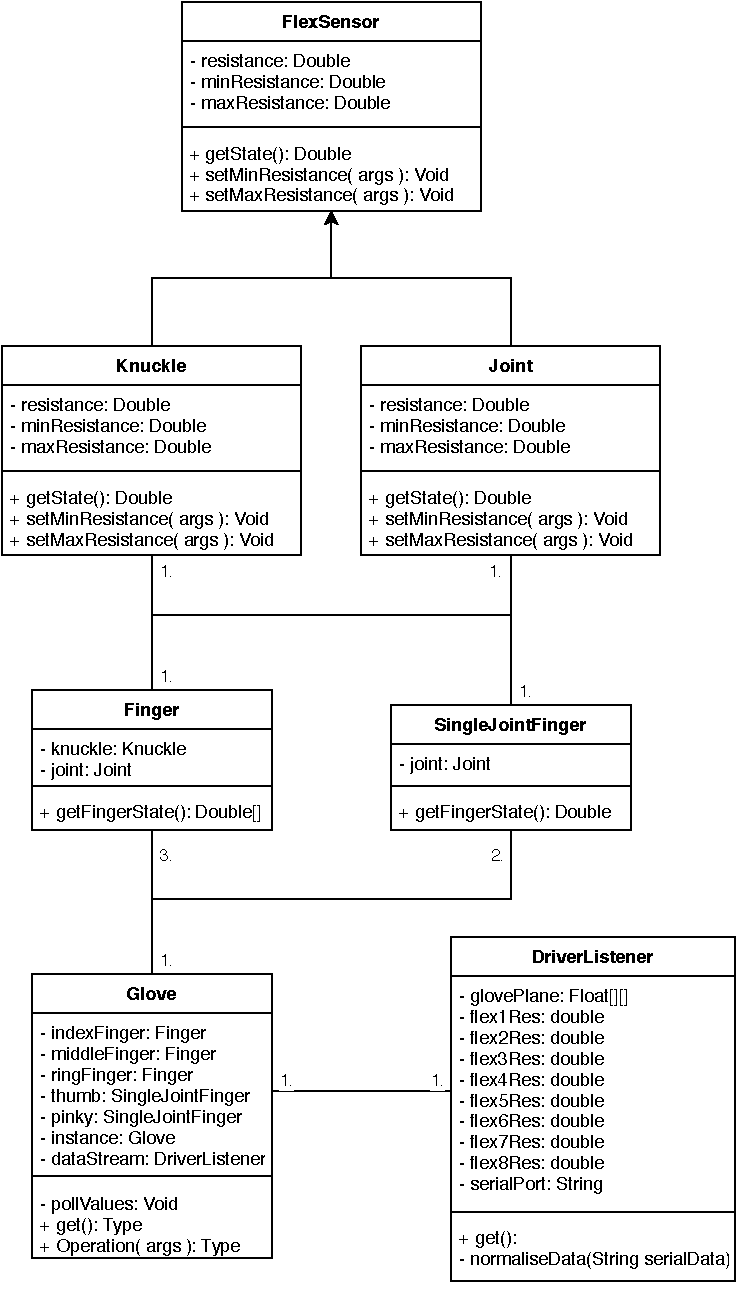
\includegraphics[]{res/UMLClassDiagram.pdf}
    \caption{UML Class Diagram}
    \label{fig:UMLClassDiagram}
\end{figure}

\chapter*{Preliminary Schedule}
\addcontentsline{toc}{chapter}{Preliminary Schedule}

\noindent In this section we will outline our provisional Gantt chart depicting how work will be completed through the duration of this project. The document is layed out as follows:

\begin{itemize}
    \item Items which are Blue will be completed by Sean Moloney.
    \item Items which are Red will be completed by Alan Devine.
    \item Items which are purple will be completed by both of us.
\end{itemize}

\noindent \textbf{Note:} Time to write unit tests is factored in with each development task presented below.

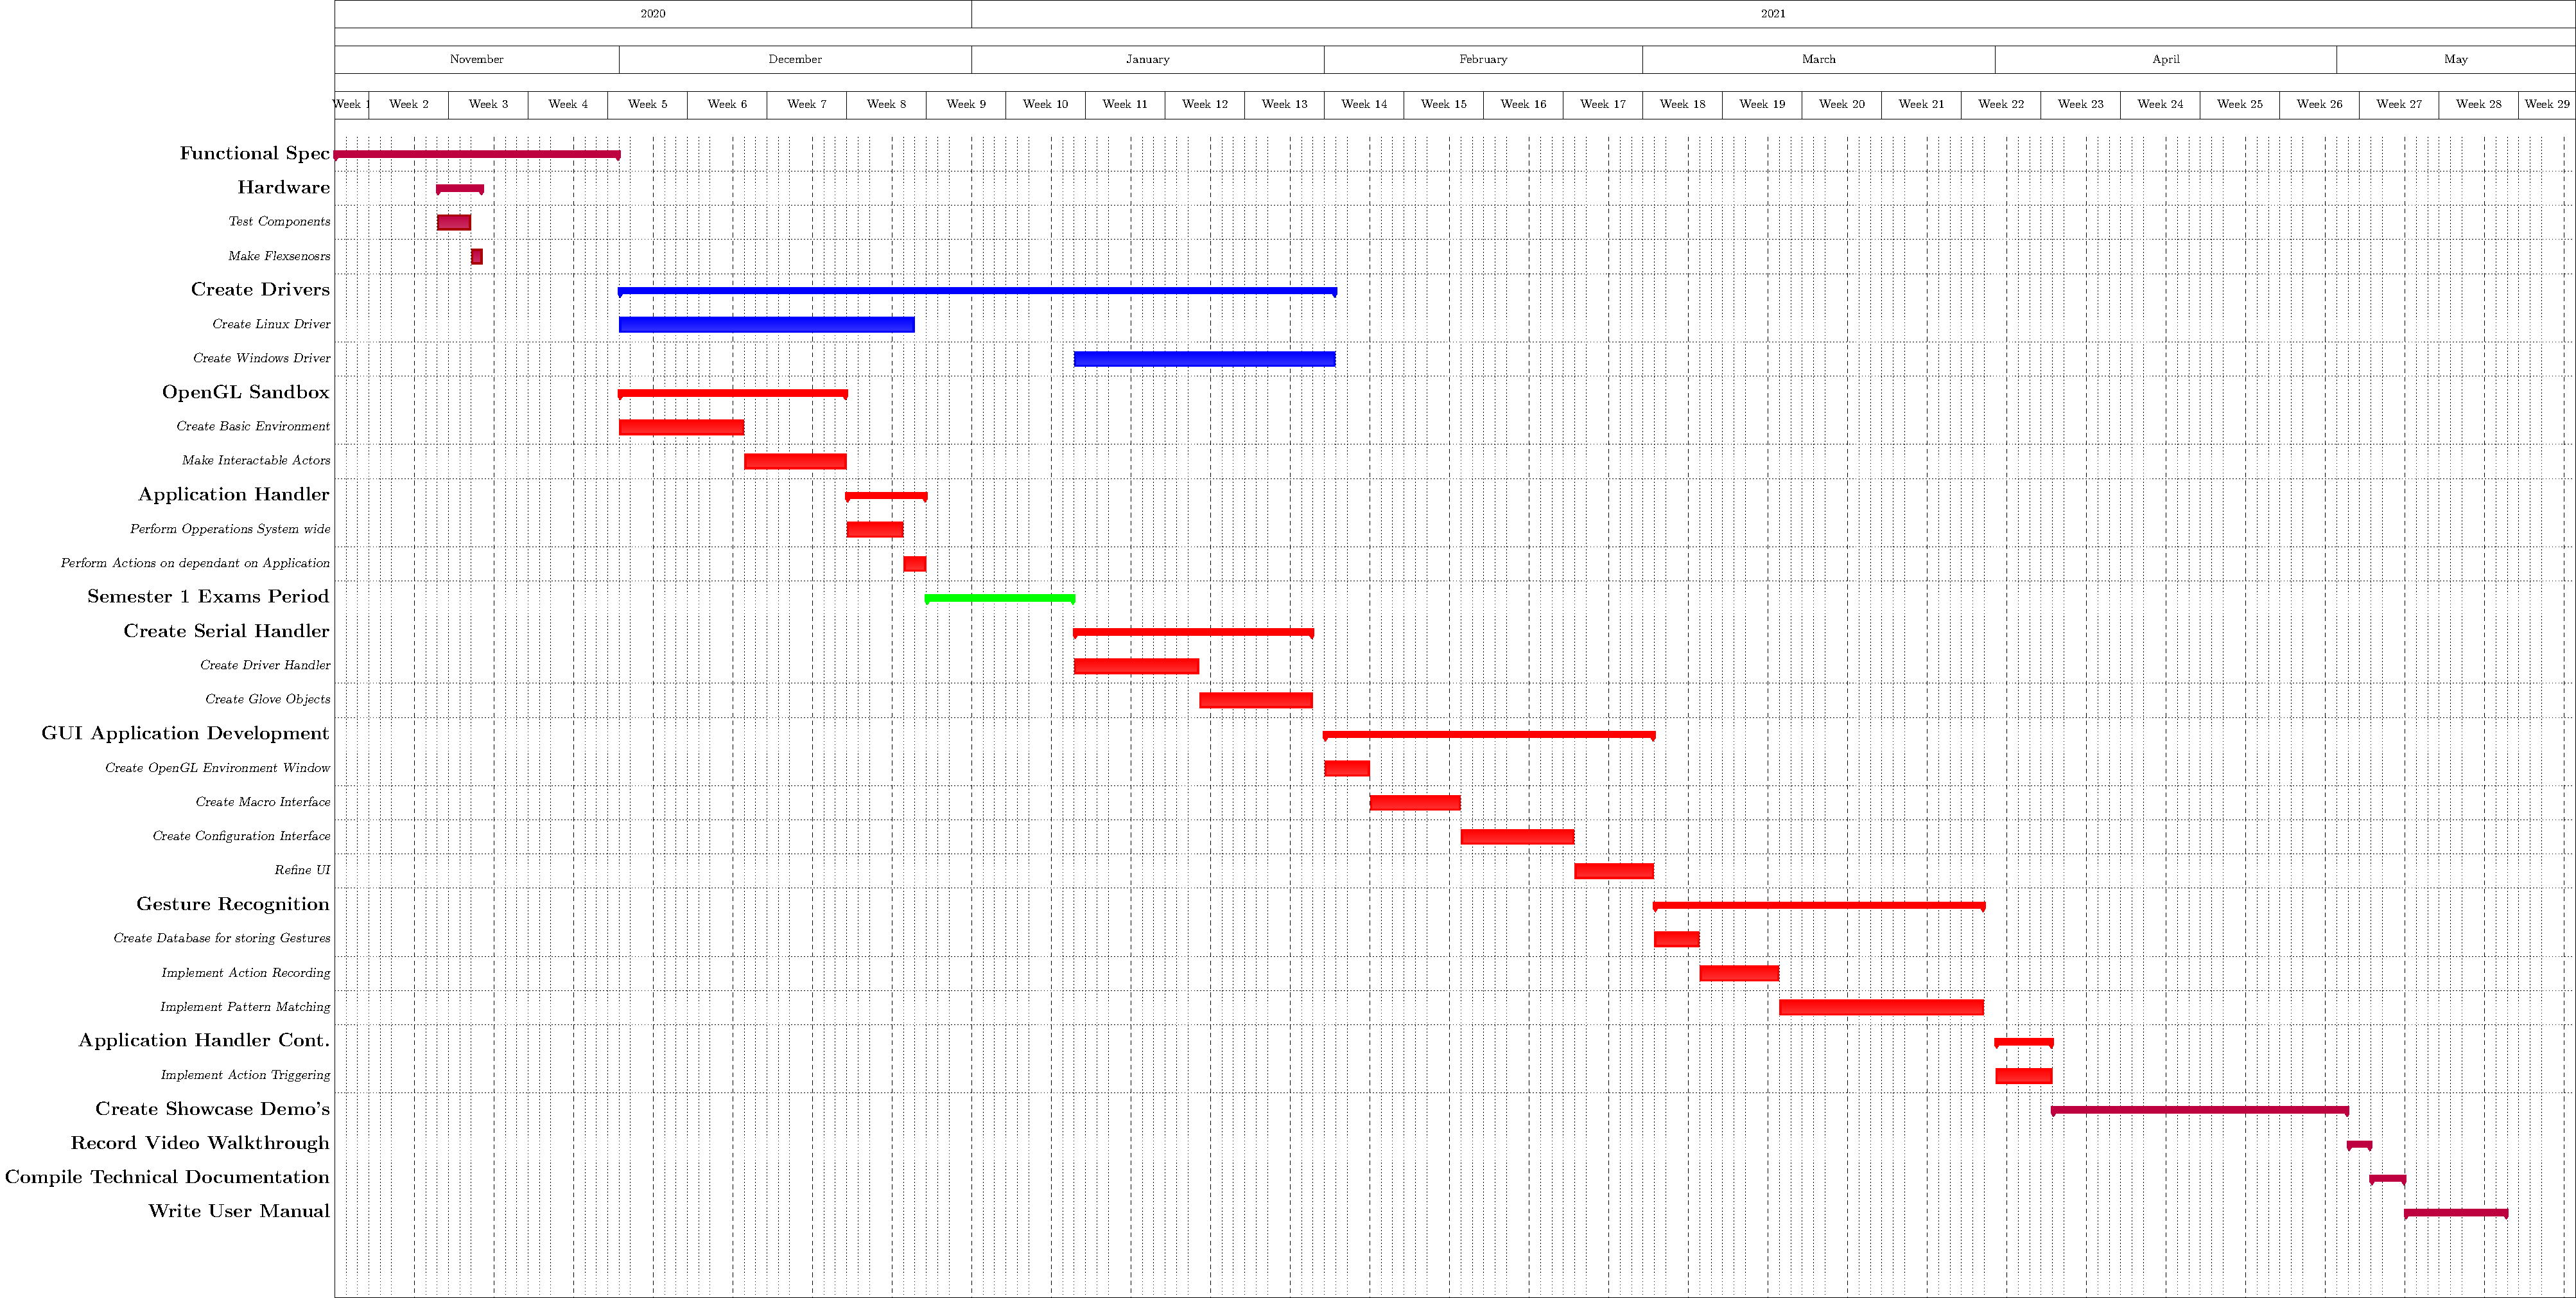
\includepdf[fitpaper=true, pages=-]{res/gantt.pdf}

\chapter*{Appendices}
\end{document}
